\documentclass[a4paper,12pt]{article}
\usepackage[utf8]{inputenc}

\usepackage[utf8]{inputenc}
\usepackage[T2A]{fontenc}
\usepackage[english,russian]{babel}
\usepackage{amsthm}
\usepackage{amsmath}
\usepackage{amssymb}
\usepackage{tikz}
\usepackage{textcomp}
\usepackage{marvosym}
\usepackage{ esint }
\usepackage{mathtext}
\usepackage{siunitx} % Required for alignment
\usepackage{subfigure}
\usepackage{multirow}
\usepackage{rotating}
\usepackage{afterpage}
\usepackage[arrowdel]{physics}
\usepackage{booktabs}
\setlength{\topmargin}{-0.5in}
\setlength{\textheight}{9.1in}
\setlength{\oddsidemargin}{-0.4in}
\setlength{\evensidemargin}{-0.4in}
\setlength{\textwidth}{7in}
\setlength{\parindent}{0ex}
\setlength{\parskip}{1ex}
\newcommand{\ndiv}{\hspace{-4pt}\not|\hspace{2pt}}
\usepackage{floatrow,graphicx,calc}
\usepackage{float}
\usepackage[export]{adjustbox}
\usepackage{wrapfig}
\usepackage{pgfplots}
\usepackage{caption}
\pgfplotsset{compat=1.16}
\graphicspath{ {./images/} }
\RequirePackage{caption}
\DeclareCaptionLabelSeparator{defffis}{ — }
\captionsetup{justification=centering,labelsep=defffis}
\usepackage{caption} \captionsetup[table]{labelsep=endash,justification=justified,singlelinecheck=false,font=normalsize}
\usepackage{amsfonts,mathtools}

\title{Лабораторная работа № 5.5.2\\Спектрометрия $\alpha$-излучения с помощью полупроводникового детектора}
\author{Илья Прамский}
\date{Декабрь 2024}

\begin{document}
\maketitle
\newpage
\section{Теоретическая справка}

Периоды полураспада $\alpha$-активных ядер очень сильно зависят от энергии вылетающих частиц. Экспериментально установленная зависимость (закон Гейгера-Нэттола) имеет вид:

\begin{equation}\label{eq:gey_net}
\lg T_{1 / 2}=\frac{a}{\sqrt{E_\alpha}}+b .
\end{equation}

Коэффициенты $a$ и $b$ очень слабо зависят от заряда ядра $Z$.

\section*{Описание установки}
В состав экспериментальной установки входит альфа-спектрометр, форвакуумный насос и персональный компьютер. (Рис. \ref{fig:scheme})

\begin{figure}[H]
  \centering
  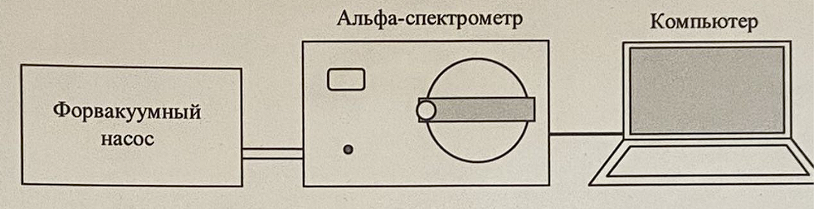
\includegraphics[width=0.8\textwidth]{scheme1.png}  \caption{Блок-схема спектрометра $\alpha$-излучения}
\end{figure}

При использовании детектора в спектрометрических целях особое значение приобретает его разрешающая способность, т. е. ширина кривой распределения импульсов по амплитудам при строго постоянной энергии регистрируемых частиц. Форма такой кривой распределения обычно бывает близка к кривой ошибок (гауссовой кривой)

\[W(U)dU = \frac{1}{\sqrt{2 \pi} \sigma} e^{\frac{-{(U-U_0)}^2}{2 \sigma^2}} dU\]

Энергетическим разрешением спектрометра обычно называют величину
\[R = \frac{\delta}{U_0} \cdot 100\%\]

Тогда связь между $\delta$ и $\sigma$:
\[\delta = 2\sqrt{2\ln 2} \sigma\]

Одной из основных причин, вызывающих разброс импульсов по амплитуде, является статистическая флуктуация числа электрондырочных пар, создаваемых падающей частицей. Среднее число пар $N$ равно

\[N = \frac{E}{\varepsilon_{\text{cp}}},\]

где $E$ - энергия, теряемая частицей в детекторе, а $\varepsilon_{\text{cp}}=3.6$ эВ - энергия, необходимая для создания пары электрон-дырка. Среднеквадратичное отклонение $\sigma$ равно

\[\sigma =\sqrt{N}=\sqrt{\frac{E}{\varepsilon_{\text{cp}}}}\]

Вклад флуктуаций числа пар в энергетическое разрешение

\[R_{\text{флук}} =\frac{\sigma}{N} \cdot 100 \% = \sqrt{\frac{\varepsilon_{\text{cp}}}{E}} \cdot 100 \%\]

\newpage
\section*{Ход работы}
Откалибруем номера каналов в энергетических единицах(МэВ).

Номера каналов, соответствующих пикам $^{226}_{88}Ra$, а также их энергия:
\begin{table}[H]
\centering
\begin{tabular}{|c|c|c|c|c|}
\hline
 & 1 пик & 2 пик & 3 пик & 4 пик \\
\hline
N канала & 1986 & 2270 & 2483 & 3168 \\
\hline
E, МэВ & 4.784 & 5.490 & 6.002 & 7.687 \\
\hline
\end{tabular}
\end{table}

\begin{figure}[H]
\centering
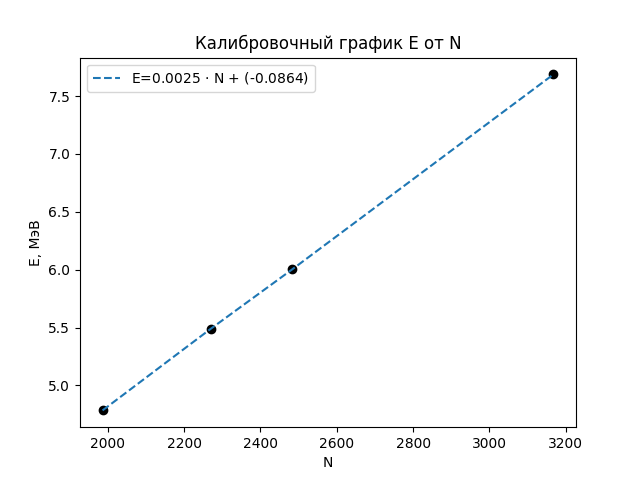
\includegraphics[scale=1]{graph1.png}
\end{figure}

\newpage
Теперь построим график зависимости счёта на сцинтилляторе $N_\text{ч}$ от энергии(Измерение для каждого из веществ были проведены за $600 \pm 5$ секунд.
\begin{figure}[H]
\centering
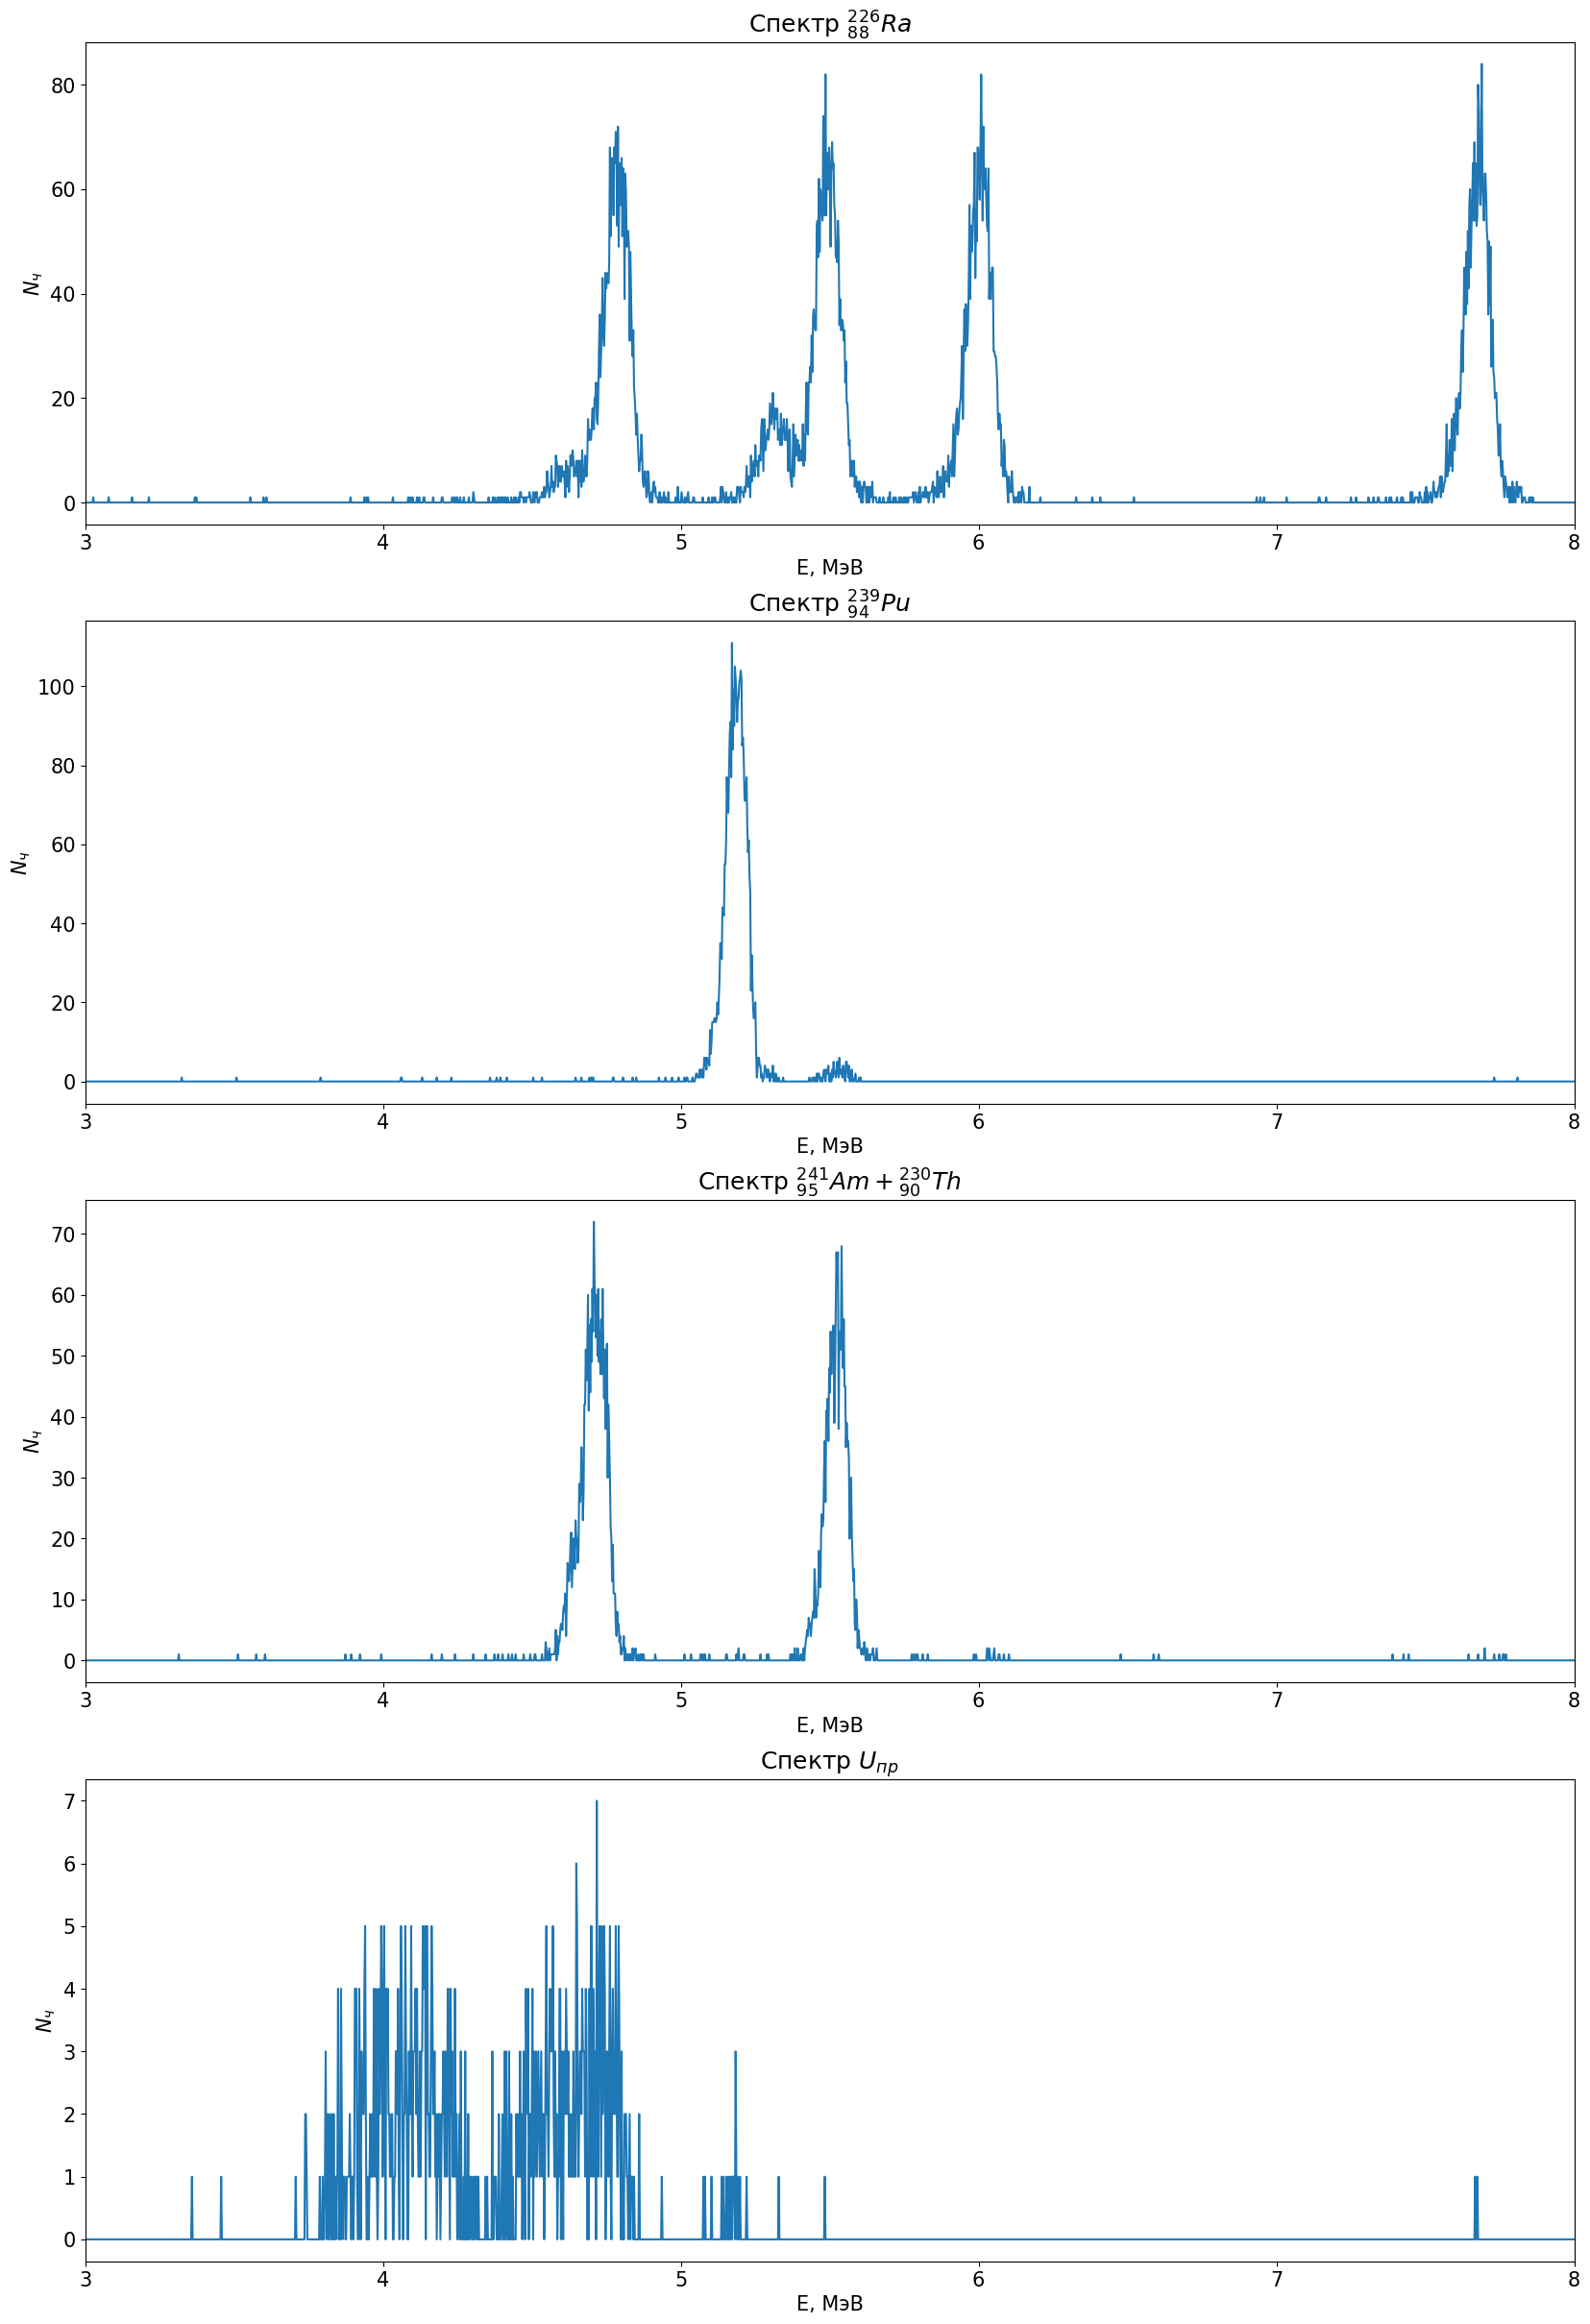
\includegraphics[scale=0.35]{graph2.png}
\end{figure}

Для каждого из веществ найдём R и заполним таблицу($N_i$ - номер канала, соответствующий пику полного поглощения, $\Delta N_i$ - ширина этого пика на половине высоты, $R_\text{эл. цеп} = R - R_\text{фл}$)

\begin{table}[H]
\begin{tabular}{|c|c|c|c|c|c|c|c|}
\hline
Источник & $N_i$ & $\Delta N_i$ & $E_i$, кэВ & $\Delta E_i$, МэВ & $R_i$, $\%$ & $R_{i,\text{фл}}, \%$ & $R_\text{эл.цеп}, \%$ \\
\hline
$^{226}_{88}Ra$ & 1986 & 37.6 & 4786.6 & 92.3 & 1.928 & 0.086 & 1.842 \\
\hline
$^{222}_{86}Rn$ & 2270 & 35.4 & 5483.5 & 86.9 & 1.585 & 0.081 & 1.504 \\
\hline
$^{218}_{84}Po$ & 2483 & 32.2 & 6006.1 & 79.0 & 1.315 & 0.077 & 1.238 \\
\hline
$^{214}_{84}Po$ & 3168 & 28.9 & 7686.9 & 70.9 & 0.922 & 0.068 & 0.854 \\
\hline
$^{239}_{94}Pu$ & 2146 & 28.0 & 5179.2 & 68.7 & 1.326 & 0.083 & 1.243 \\
\hline
$(\text{доч.}) ^{239}_{94}Pu$ & 2290 & 30.0 & 5532.5 & 73.6 & 1.330 & 0.081 & 1.250 \\
\hline
$^{241}_{95}Am + ^{230}_{90}Th$ & 1953 & 34.9 & 4705.6 & 85.6 & 1.819 & 0.087 & 1.732 \\ 
\hline
$(\text{доч.}) ^{241}_{95}Am + ^{230}_{90}Th$ & 2287 & 26.6 & 5525.2 & 65.3 & 1.182 & 0.081 & 1.101 \\
\hline
$U_\text{пр}$ & 1690 & 53 & 4060.3 & 130.0 & 3.202 & 0.094 & 3.108 \\
\hline
$(\text{доч.}) U_\text{пр}$ & 1930 & 80 & 4649.2 & 196.3 & 4.222 & 0.088 & 4.134 \\
\hline
\end{tabular}
\end{table}

Теперь проверим закон Гейгера-Неттола для $^{226}_{88}Ra$ и его дочерних ядер.
\begin{table}[H]
\centering
\begin{tabular}{|c|c|c|c|c|}
\hline
Вещество & $^{226}_{88}Ra$ & $^{222}_{86}Rn$ & $^{218}_{84}Po$ & $^{214}_{84}Po$ \\
\hline
T, & 1620 лет & $3.82$ суток & $3.11$ минут & $1.63 \cdot 10^{-4}$ секунд \\
\hline
E, кэВ & 4786.6 & 5483.5 & 6006.1 & 7686.9 \\
\hline
\end{tabular}
\end{table}

\begin{figure}[H]
\centering
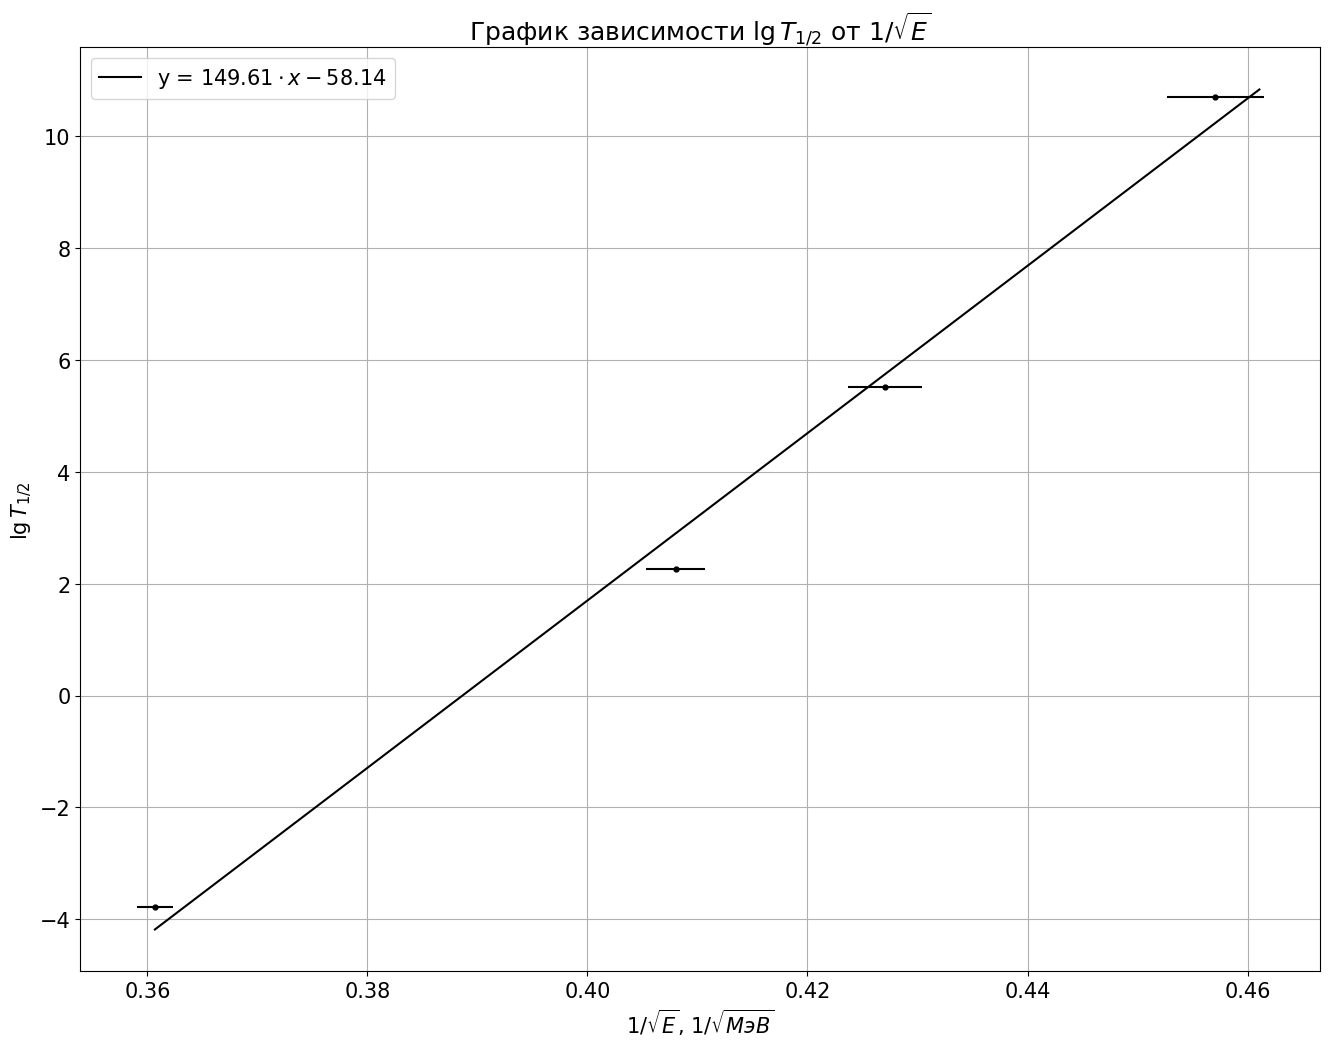
\includegraphics[scale=0.5]{graph3.png}
\end{figure}
Получается $a_\text{эксп} = 150 \pm 9 \sqrt{\text{МэВ}}$, $b_\text{эксп} = -58 \pm 4$.

$a_\text{т} = 147 \sqrt{\text{МэВ}}$, $b_\text{т} = -54$

\section*{Вывод}
В ходе работы былы исследован энергетический спектр $\alpha$-частиц при распаде различных веществ, также для каждого пика было вычислено энергетическое разрешение. Помимо этого был также проверен закон Гейгера-Неттола на $^{226}_{88}Ra$ и его дочерних ядрах.
\end{document}